% 质心 质心系

\pentry{体积分\upref{IntN}, 质点系\upref{PSys}}

\subsection{质心的定义}
质心通俗来讲可以理解为质量的中心, 是系统中各个质点的位置矢量\upref{Disp}关于质量的加权平均值. 我们先看几个例子.

\subsection{两个等质量质点的质心}
对于两个质量相等的质点, 它们的质心显然在它们连线的中点处, 无论它们的质量是多少. 如果它们都在 $x$ 轴上, 则质心的位置就是两质点 $x$ 坐标的中点
\begin{equation}\label{CM_eq2}
x_c = (x_1 + x_2)/2
\end{equation}
其中角标 c 表示 center of mass, 有时候也会写做 CM.

在二维和三维空间的情况下, 质点的位置用位置矢量 $\vec r$ 描述, 将它们的位置矢量分别记为 $\vec r_1$ 和 $\vec r_2$, 则质心的位置为
\begin{equation}\label{CM_eq3}
\vec r_c = (\vec r_1 + \vec r_2)/2
\end{equation}
即两个位置矢量的平均值. % 图未完成

\subsection{两个不同质量质点的质心}
当两个质点质量不一样时(分别记为 $m_1$ 和 $m_2$), 质心会更靠近更重的质点. 如果它们都在 $x$ 轴上, 我们就用加权平均值
\begin{equation}
x_c = \frac{m_1 x_1 + m_2 x_2}{m_1 + m_2}
\end{equation}
注意 $m_1 = m_2$ 就得到了\autoref{CM_eq1}. 另一个极端是当一个质量远大于另一个, 如 $m_1 \gg m_2$, 这时质心就趋近于 $x_1$ 了.

二维和三维空间的情况下也类似有
\begin{equation}\label{CM_eq5}
\vec r_c = \frac{m_1 \vec r_1 + m_2 \vec r_2}{m_1 + m_2}
\end{equation}
当 $m_1 = m_2$ 就得到\autoref{CM_eq3}.

\begin{exer}{}
证明两质点的质心必定在其连线上, 即 $\vec r_1 - \vec r_c$ 和 $\vec r_2 - \vec r_c$ 共线。% 共线如何证明? “几何矢量” 中有提吗?
\end{exer}

\begin{exer}{}
试证明\autoref{CM_eq5} 中质心到两质点的距离与它们的质量成反比, 即
\begin{equation}\label{CM_eq6}
\frac{\abs{\vec r_1 - \vec r_c}}{\abs{\vec r_2 - \vec r_c}} = \frac{m_2}{m_1}
\end{equation}
\end{exer}

\subsection{质点系}
若质点系中有 $N$ 个质点,令第 $i$ 个质点质量为 $m_i$,位置为 $\vec r_i$,总质量为 $M = \sum\limits_i m_i$, 则该质点系的\bb{质心}定义为
\begin{equation}\label{CM_eq1}
\vec r_c = \frac{1}{M}\sum_i m_i \vec r_i
\end{equation}

\subsection{质心的分解}
若我们把质点系划分为若干组, 可以先计算每组的质心, 再计算 “质心的质心” 就可以得到系统的总质心。 我们举例说明
\begin{exam}{}
令四个质点中的前两个为 a 组, 后两个为 b 组, 则它们的质心分别为
\begin{equation}
\vec r_a = (m_1 \vec r_1 + m_2 \vec r_2)/M_a
\qquad
\vec r_b = (m_3 \vec r_3 + m_4 \vec r_4)/M_b
\end{equation}
其中 $M_a = m_1 + m_2$, $M_b = m_3 + m_4$。 再计算 “质心的质心” 得整个系统的质心为
\begin{equation}
\vec r_c = \frac{M_a \vec r_a + M_b \vec r_b}{M_a + M_b} = \frac{m_1 \vec r_1 + m_2 \vec r_2 + m_3 \vec r_3 + m_4 \vec r_4}{m_1 + m_2 + m_3 + m_4}
\end{equation}
这恰好符合\autoref{CM_eq1}。
\end{exam}

\subsection{质心与重心}
我们只讨论均匀引力场中物体的重心。 其定义是: 若重力场对物体关于某点的合力矩恒为 0, 这个点就是它的\bb{重心}。 “合力矩为零” 意味着, 如果物体初始时静止, 那么它将一直保持静止。 虽然我们还没系统学习力矩, 但可以用初中学过的 “力乘力臂” 进行计算(\autoref{Torque_eq2}\upref{Torque})。

\begin{exam}{}\label{CM_ex1}
\begin{figure}[ht]
\centering
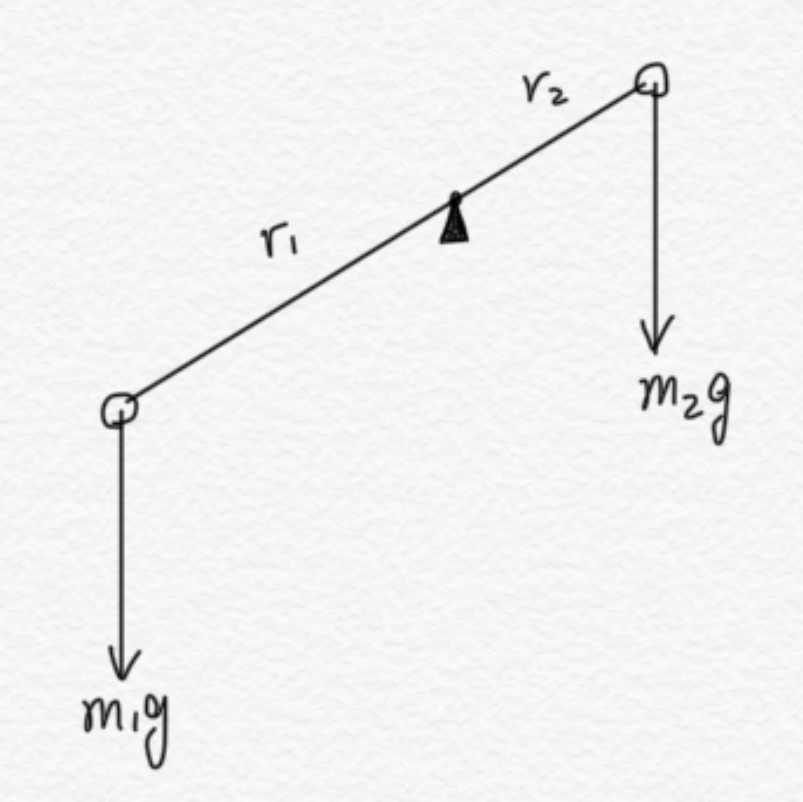
\includegraphics[width=5.5cm]{./figures/CM1.png}
\caption{轻杆与两小球} \label{CM_fig1}
\end{figure}

轻杆\footnote{轻杆是指质量可忽略不计的杆}两端有质量分别为 $m_1$ 和 $m_2$ 的小球, 轻杆可以绕系统质心在竖直平面上自由转动。 试证明重力对系统的力矩恒为 0。

解: 以逆时针为正, 合力矩为
\begin{equation}
M = r_1 m_1 g \cos\theta - r_2 m_2 g \cos\theta = (r_1 m_1 - r_2 m_2) g \cos\theta
\end{equation}
由\autoref{CM_eq6}, 括号中两项相等, 所以无论 $\theta$ 去何值, 合力矩都为 0。
\end{exam}
我们把一般性的证明留到 “重心\upref{CenG}” 中。

\subsection{连续质量分布}
% 未完成: 三角形的质心, 扇形的质心
对连续质量分布,令密度关于位置的函数为 $\rho (\vec r)$,总质量为密度的体积分 %(链接未完成)
\begin{equation}
M = \int \rho (\vec r) \dd{V}
\end{equation}
质心定义为
\begin{equation}
\vec r_c = \frac{1}{M}\int \vec r\rho (\vec r) \dd{V}
\end{equation}
以下的讨论都对质点系进行,连续质量分布可看做由许多体积微元组成,也可看做质点系.

\subsection{质心的唯一性}
既然质心的定义取决于参考系(因为 $\vec r_i$ 取决于参考系),那么不同参考系中计算出的质心是否是空间中的同一点呢?我们只需要证明,在 $A$ 坐标系中得到的质心 $\vec r_{Ac}$ 与 $B$ 坐标系中得到的质心 $\vec r_{Bc}$ 满足关系
\begin{equation}\label{CM_eq4}
\vec r_{Ac} = \vec r_{AB} + \vec r_{Bc}
\end{equation}
其中 $\vec r_{AB}$ 是 $A$ 系原点指向 $B$ 系原点的矢量. 首先根据定义
\begin{equation}
\vec r_{Ac} = \frac{1}{M}\sum_i m_i \vec r_{Ai}  \qquad \vec r_{Bc} = \frac{1}{M}\sum_i  m_i \vec r_{Bi} 
\end{equation}
由位矢的坐标系变换%(未完成: 确保有介绍)
,$\vec r_{Ai} = \vec r_{AB} + \vec r_{Bi}$, 所以
\begin{equation}
\vec r_{Ac} = \frac{1}{M}\sum_i m_i(\vec r_{AB} + \vec r_{Bi})  = \vec r_{AB} + \frac{1}{M} \sum_i m_i \vec r_{Bi}  = \vec r_{AB} + \vec r_{Bc}
\end{equation}
 
\subsection{质心系}
定义质点系的\bb{质心系}为原点固定在质心上且没有转动的参考系(平动参考系).%链接未完成: 平动是相对的, 转动是绝对的.
根据质心的唯一性(\autoref{CM_eq4}),在质心系中计算质心(\autoref{CM_eq1}) 仍然落在原点,即
\begin{equation}\label{CM_eq7}
\sum_i m_i \vec r_{ci} = \vec 0
\end{equation}
其中 $\vec r_{ci}$ 是质心系中质点 $i$ 的位矢.

注意质心系并不一定是惯性系,只有当合外力为零质心做匀速直线运动时,质心系才是惯性系.在非惯性系中,每个质点受惯性力.

\subsection{质心系中总动量}
把\autoref{CM_eq7} 两边对时间求导,得
\begin{equation}\label{CM_eq8}
\sum_i m_i \vec v_{ci} = \vec 0
\end{equation}
注意到等式左边恰好为质心系中质点系的总动量,所以我们得到质心系的一个重要特点,\bb{质心系中总动量为零}.
